\documentclass[11pt,a4paper]{report}

\usepackage{geometry}
\usepackage{graphicx}
\usepackage{longtable}
\usepackage{pgfgantt}
\usepackage[dutch]{babel}
\usepackage{url}
\usepackage{pgf,pgfplots}
\usetikzlibrary{fit,calc}
\usepgfplotslibrary{external}

\geometry{a4paper}

\newcommand{\boxplot}[6]{%
	%#1: center, #2: median, #3: 1/4 quartile, #4: 3/4 quartile, #5: min, #6: max
	\filldraw[fill=white,line width=0.2mm] let \n{boxxl}={#1-0.1}, \n{boxxr}={#1+0.1} in (axis cs:\n{boxxl},#3) rectangle (axis cs:\n{boxxr},#4);   % draw the box
	\draw[line width=0.2mm, color=red] let \n{boxxl}={#1-0.1}, \n{boxxr}={#1+0.1} in (axis cs:\n{boxxl},#2) -- (axis cs:\n{boxxr},#2);             	% median
	\draw[line width=0.2mm] (axis cs:#1,#4) -- (axis cs:#1,#6);                                                                           							% bar up
	\draw[line width=0.2mm] let \n{whiskerl}={#1-0.025}, \n{whiskerr}={#1+0.025} in (axis cs:\n{whiskerl},#6) -- (axis cs:\n{whiskerr},#6);        % upper quartile
	\draw[line width=0.2mm] (axis cs:#1,#3) -- (axis cs:#1,#5);                                                                           							% bar down
	\draw[line width=0.2mm] let \n{whiskerl}={#1-0.025}, \n{whiskerr}={#1+0.025} in (axis cs:\n{whiskerl},#5) -- (axis cs:\n{whiskerr},#5);        % lower quartile
}

\title{P\&O Computerwetenschappen - Verslag}
\author{Team Platinum}

\begin{document}

\maketitle
\tableofcontents

\begin{abstract}
Tijdens de uitwerking van dit groepswerk, bouwen wij een autonome robot met behulp van Lego Mindstorms. Voor de programmatie wordt beroep gedaan op Lejos, een Open Bron project dat een minimale JAVA virtuele machine heeft gemaakt die de plaats kan innemen van de standaard programmatie omgeving van Lego.

Naast de doelstelling om kennis te maken met het ontwikkelen van een autonome robot, willen we in dit project ook ervaring opdoen ivm het werken in team verband aan een middelgroot softwareproject. Hierbij zijn organisatie van werk, planning, analyse, architectuur,... belangrijke begrippen.

Parallel met het verplicht te volgen traject van meerdere demo sessies, kiezen we voor een traject waarbij het uiteindelijke doel van het project voorop wordt gesteld: een volledig onbekend traject autonoom afleggen. Hiertoe hebben we om een vlotte integratie mogelijk te maken, na een korte analyse, interfaces afgesproken, waar beide trajecten zich aan houden.

In het parallelle traject ontwikkelen we een simulatieomgeving. Aan de hand van deze omgeving zijn we in staat om met meerdere teamleden in parallel te werken aan de software voor de robot, zonder nood aan een fysieke versie voor elk van de leden. Een tweede voordeel ligt in de snelheid waarmee een virtuele robot zich op een virtueel parcours kan bewegen, wat het wachten tot een minimum beperkt. Tot slot is de flexibiliteit om met de debugger van een IDE door de logica van de robot te kunnen stappen van onschatbare waarde.
\end{abstract}

\chapter{Inleiding}

De tussentijdse demos helpen om de technologie stapsgewijs te verkennen. Geen van deze tussenstappen is echter rechtstreeks inzetbaar bij het effectieve doel: het autonoom rijden van een onbekend traject.

We kiezen er voor om ons team op te splitsen en twee verschillende trajecten te volgen: \'e\'en dat zich toelegt op het optimaal implementeren van de tussentijdse opdrachten en \'e\'en dat er voor zorgt dat een volledige architectuur uitgewerkt wordt die ons zal toelaten om de eindopdracht optimaal te realiseren.

Op basis van een architectuur studie werden de componenten van de eindoplossing ge\"identificeerd. In een Work Breakdown Structure\footnote{\url{http://en.wikipedia.org/wiki/Work_breakdown_structure}} (WBS) werden vervolgens de deelstappen opgelijst, toegewezen aan verantwoordelijken en er werden deadlines bepaald. Deze informatie vormde de basis voor een planning. De WBS en planning zijn opgenomen in respectievelijk bijlagen \ref{appendix:wbs} en \ref{appendix:planning}

\section{Architectuur}

De architectuur die we zullen implementeren in dit project richt zich op het realiseren van een robuuste oplossing; zowel op het vlak van de autonome robot als ook op het volledige framework er rond dat we opbouwen op de PC. Figuur \ref{fig:architectuur} geeft de algemene architectuur weer. We belichten vervolgens de architectuur vanuit het oogpunt van beide omgevingen waar de oplossing zal actief zijn: de robot en de PC.

\begin{figure}[htbp]
   \centering
   \includegraphics[width=200mm, angle=90]{resources/architectuur.pdf}
   \caption{Architectuur}
   \label{fig:architectuur}
\end{figure}

\subsection{Robot}

De robot biedt een technische API die toegang verleent tot de motoren en sensoren. We kiezen er voor om een eigen RobotAPI te introduceren die abstractie maakt van de technische API. Deze zal ons toelaten een andere implementatie te maken, die binnen een gesimuleerde omgeving gebruikt kan worden. Met deze omgeving kunnen we de logica van de robot ontwikkelen zonder een fysieke robot.

Een tweede belangrijke component binnen de robot is de �Main Event Loop�\footnote{\url{http://en.wikipedia.org/wiki/Event_loop}}. We hergebruiken hier een term die uit de wereld van de grafische gebruikers interfaces komt, maar zeer goed weergeeft wat hier gebeurt. De Main Event Loop doorloopt eindeloos 5 stappen: 

\begin{enumerate}
\item haal gegevens op van alle sensoren
\item voed de gegevens in het model
\item ondervraag de navigator welke acties dienen ondernomen te worden
\item de navigator consulteert het model om de volgende acties te bepalen
\item voer de acties uit door middel van de robot API
\end{enumerate}

Het model is een interne voorstellingsvorm van de wereld waarin de robot zich bevindt. Aan het begin van de Event Loop zal dit model leeg zijn. Met leeg bedoelen we volledig onbekend. Gaandeweg zal op basis van de input van de sensoren dit model gevoed worden en zal een wereldbeeld ontstaan met verschillende graden van zekerheid.

De navigator consulteert vervolgens dit model om de volgende actie te bepalen en implementeert op deze manier het ``doel'' van de robot. Deze acties worden uitgedrukt in de taal van de RobotAPI en bestaan uit functionele opdrachten zoals beweeg $x$ meter vooruit of draai $x$ graden. 

Naast de Main Event Loop voorzien we een tweede onafhankelijke Event Loop voor de communicatie met de PC. Deze geschiedt via Bluetooth. De redenen om deze gescheiden te houden zijn triviaal: enerzijds willen we de werking van de robot zelf niet onnodig in gevaar brengen met een proces dat kan falen. Anderzijds zal ook de frequentie waarop beide processen opereren niet gelijk lopen.

Een voorbeeld hiervan is de stroom van informatie die de lichtsensoren of sonar zullen aanbieden. Het volledig overzenden van deze gegevens kan eventueel niet mogelijk (te veel voor de beschikbare bandbreedte) of niet wenselijk (onnuttige informatie) zijn.

\subsection{PC}

Op de PC wordt alle communicatie met de robot verzorgd langs een zgn. Robot Agent. Deze extra laag zal de robuustheid van de oplossing verhogen, door het beperken van synchroon uitgevoerde code. We denken hierbij aan het rechtstreeks koppelen van de communicatie aan een gebruikersinterface.

We zijn van mening dat het louter verzenden en visualiseren van informatie over de werking van de robot een verlies aan mogelijkheden zou betekenen. Onze strategie gebaseerd op een simulatieomgeving toont al snel aan dat deze informatie kan helpen bij het onderzoek naar optimale navigator-logica.

Aangezien we de informatie dus wensen te bewaren, willen we dit ook een centraal gegeven van onze architectuur maken. Opnieuw komt dit de robuustheid van de gehele oplossing ten goede. De focus zal komen te liggen op het optimaal opslaan van de gegevens. Het visualiseren komt vervolgens neer op het consulteren van de opgeslagen gegeven. Dit is opnieuw een volledig asynchroon proces tov. de robot.

Deze architectuur heeft enkele bijkomende gevolgen. Het is bvb. mogelijk om gegevens van meerdere sessies simultaan te bekijken of kan met meerdere en/of verschillende gebruikersinterfaces gewerkt worden. Ook kan voor de realisatie van deze architectuur beroep gedaan worden op enkele standaarden, waardoor het cre\"eren van nieuwe code tot een minimum beperkt wordt.

De Log Server kan ge\"implementeerd worden op basis van log4j\footnote{\url{http://logging.apache.org/log4j/}} en kan de aflevering van de inkomende communicatie volledig in configuratie gerealiseerd worden. De meest eenvoudige uitwerking kan bestaan uit het gebruiken van een syslog daemon, maar ook een relationele databank is triviaal.

Verschillende types clients kunnen de gegevens uit de databank visualiseren: een Fat Client\footnote{\url{http://en.wikipedia.org/wiki/Fat_client}} ligt voor de hand, maar ook een webapplicatie of REST\footnote{\url{http://en.wikipedia.org/wiki/Representational_state_transfer}}-service zijn goede opties.

Deze laatste kan dan opnieuw gerealiseerd worden gebruikmakend van standaard componenten zoals de JBoss applicatie server\footnote{\url{http://www.jboss.org/jbossas}} en RESTeasy\footnote{\url{http://www.jboss.org/resteasy}}. Door middel van long polling\footnote{\url{http://en.wikipedia.org/wiki/Push_technology#Long_polling}} kan zelfs op heel eenvoudig wijze een streaming oplossing aan web-clients aangeboden worden.

\subsection{Interactie}

De architectuur (figuur \ref{fig:architectuur}) voorziet eveneens de mogelijkheid om commando's te sturen naar de robot. Aan de zijde van de robot zullen de meeste van de componenten handelingen registreren bij de communicatiecomponent. Op deze manier kunnen de commando's door de communicatie component uitgevoerd worden op de geregistreerde handelingen op de componenten. Dit stelt ons in staat om op generieke manier interactief de software van de robot te ondervragen, zonder specifieke code te moeten voorzien.

\section{Functionele Analyse}

In de functionele analyse bepalen we in hoofdzaak de interfaces die gerespecteerd dienen te worden in de twee trajecten. Op basis van deze afspraken kunnen beide trajecten integreren en in elkaar opgaan.

Twee interfaces worden voorzien: de Robot interface en de RobotAPI interface. De eerste bepaalt hoe de robot opgebouwd en aangesproken kan worden door zijn omgeving. Dit kan een programma zijn dat op de robot uitgevoerd wordt, of dit kan een simulatieomgeving zijn. Ook op niveau van de RobotAPI moet deze mogelijkheid beschikbaar zijn. Figuur \ref{fig:robotapi} toont de high-level specificatie waar alles verder rond gebouwd is. De combinatie van de Robot en RobotAPI interface lieten ons toe om verschillende robots te construeren die zowel in de echte wereld als in een simulatieomgeving zonder enige aanpassing konden werken.

\begin{figure}[htbp]
   \centering
   \includegraphics[width=150mm]{resources/model-robot.png}
    \caption{Robot \& RobotAPI Interfaces en hun implementaties.}
   \label{fig:robotapi}
\end{figure}

\chapter{Demo 1: Veelhoek}

De doelstelling van de eerste demo is het rijden van een veelhoek op basis van het aantal hoeken en de lengte van een zijde. Precisie door middel van compensatie van de vast te stellen afwijkingen is hier van belang.

\section{Fysiek ontwerp}

Het ontwerp van de robot voor de eerste opdracht is het basismodel van de Mindstorms kit die we ter beschikking kregen. Gegeven het korte tijdsbestek was het belangrijker om snel ervaring op te doen met de robot. Deze ervaring kan eveneens informatie verschaffen aan het lange termijn traject.
 
\section{De software}
 
De Lejos API biedt twee mogelijkheden om de motoren aan te sturen: op basis van tijd en op basis van de omwentelingen van de wielen. Intu\"itief waren we ervan overtuigd dat de methode op basis van omwentelingen de meest betrouwbare moest zijn.

Wat betreft de rij-technische mogelijkheden, kiezen we voor twee onafhankelijke bewegingen: het rechtdoor rijden (vooruit of achteruit) en het ter plekke draaien. Dit is enerzijds een noodzaak voor de opdracht, maar is tevens de eenvoudigste te hanteren en betrouwbaarste methode. Het draaien tijdens het rijden gaat gepaard met noodzakelijke slip- en schuifbewegingen, wat de berekenbaarheid sterk kan be"invloeden.

In beide gevallen is er nog een parameter die bepalend kan zijn: de rotatiesnelheid. Ook deze zullen we in onze testen laten vari\"eren om een optimale verhouding te vinden.

\section{Testplan en resultaten}

\subsection{Omwentelingen}

De implementatie die omwentelingen telt, is afhankelijk van de omtrek van de wielen. De theoretische omtrek van het wiel kan berekend worden op basis van de diameter (56mm) en bedraagt 175,93mm.

Naast de theoretische bepaling van de omtrek voorzien we ook software die deze omtrek bepaalt op basis van een zgn. zelf-calibratie. Hierbij laten we de robot rijden, voorzien van een frontale druksensor, tot hij een obstakel raakt. Op dit ogenblik stop de robot. Vervolgens nemen we de blokkade weg en zal de robot na enkele seconden zelf verder rijden tot het volgende obstakel. Op basis van de getelde omwentelingen en de vaste afstand tussen beide obstakels, kan de robot vervolgens zelf exact de omtrek van het wiel bepalen.

De waarde die op deze manier werd vastgesteld was 175mm. Deze werd gebruikt als initi\"ele waarde.

\subsubsection{Test 1: met een vaste snelheid verschillende afstanden rijden}

Voor deze test werd de snelheid ingesteld op 400 en werden afstanden van 20, 40, 60 en 80 cm gereden. Bij de uiteindelijke opdracht wordt er gereden op een parcours dat bestaat uit panelen van 80 bij 80 cm. De robot zal zelden grotere afstanden aan \'e\'en stuk rijden.

We lieten de robot telkens 5 maal de vooropgestelde afstand rijden en berekenden vervolgens de relatieve afwijkingen. De resultaten van deze test zijn opgenomen in figuur \ref{chart:test1}.

\begin{figure}
	\caption{Test 1 : Relatieve afwijking bij vaste snelheid}
	\label{chart:test1}
	\vspace{10pt}	
	\centering
	
	\tikzset{external/remake next}
	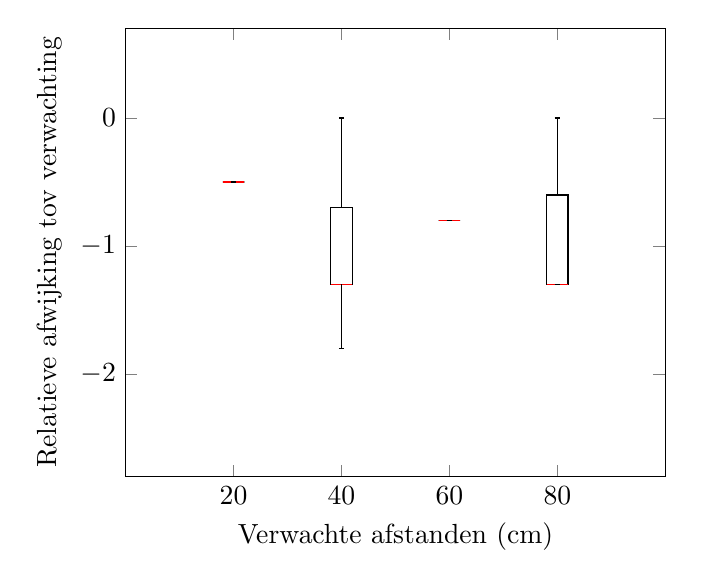
\begin{tikzpicture}
		\begin{axis}[xmin=0,xmax=5,ymin=-2.8, ymax=0.7,
			xtick={1,2,3,4,5},xticklabels={20,40,60,80},
	      		xlabel={Verwachte afstanden (cm)},
			ylabel={Relatieve afwijking tov verwachting},
			]
			%#1: center, #2: median, #3: 1/4 quartile, #4: 3/4 quartile, #5: min, #6: max
			\boxplot{1}{-0.5}{-0.5}{-0.5}{-0.5}{-0.5}
			\boxplot{2}{-1.3}{-1.3}{-0.7}{-1.8}{0}
			\boxplot{3}{-0.8}{-0.8}{-0.8}{-0.8}{-0.8}
			\boxplot{4}{-1.3}{-1.3}{-0.6}{-1.3}{0}
		\end{axis}
	\end{tikzpicture}
\end{figure}

Op basis van de resultaten, werd de wielomtrek met 1\% verkleind. Figuur \ref{chart:test1b} toont de resultaten van dezelfde test na de aanpassing.

\begin{figure}
	\caption{Test 1 : Resultaten na aanpassing wielomtrek met 1\%}
	\label{chart:test1b}
	\vspace{10pt}	
	\centering
	
	\tikzset{external/remake next}
	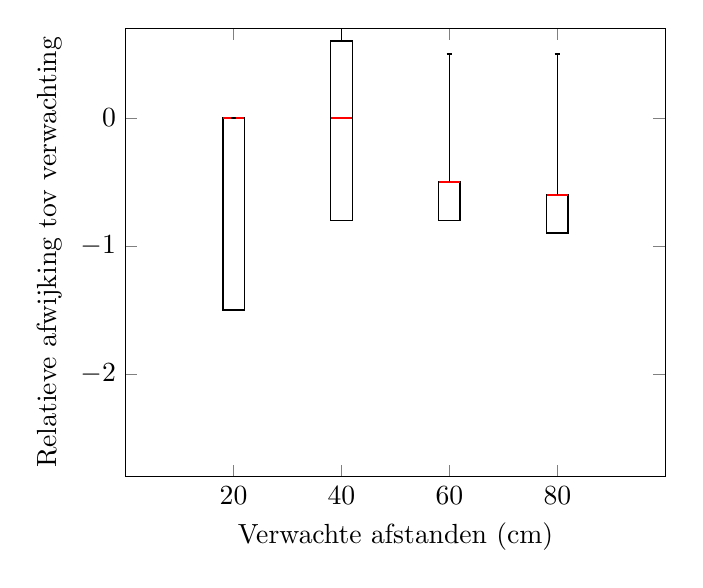
\begin{tikzpicture}
		\begin{axis}[xmin=0,xmax=5,ymin=-2.8, ymax=0.7,
			xtick={1,2,3,4,5},xticklabels={20,40,60,80},
	      		xlabel={Verwachte afstanden (cm)},
			ylabel={Relatieve afwijking tov verwachting},
			]
			%#1: center, #2: median, #3: 1/4 quartile, #4: 3/4 quartile, #5: min, #6: max
			\boxplot{1}{0}{-1.5}{0}{-1.5}{0}
			\boxplot{2}{0}{-0.8}{0.6}{-0.8}{0.8}
			\boxplot{3}{-0.5}{-0.8}{-0.5}{-0.8}{0.5}
			\boxplot{4}{-0.6}{-0.9}{-0.6}{-0.9}{0.5}
		\end{axis}
	\end{tikzpicture}
\end{figure}

\subsubsection{Test 2: een vaste afstand met verschillende snelheden}

Bij het uitvoeren van verkennende testen hadden we reeds vastgesteld dat het vertrekken, stoppen en de snelheid van de motoren een beduidende invloed hadden op de stabiliteit van de robot. Met deze tweede test willen we op zoek gaan naar een optimale snelheid/precisie verhouding.

We lieten de robot telkens 5 maal een afstand van 20cm afleggen bij vari\"erende motorsnelheden: 125, 250, 500, 750 en 1000. Vervolgens  berekenden we de relatieve afwijking. De resultaten van deze test zijn opgenomen in figuur \ref{chart:test2}.

\begin{figure}
	\caption{Test 2 : Relatieve afwijking bij variabele snelheden}
	\label{chart:test2}
	\vspace{10pt}	
	\centering
	
	\tikzset{external/remake next}
	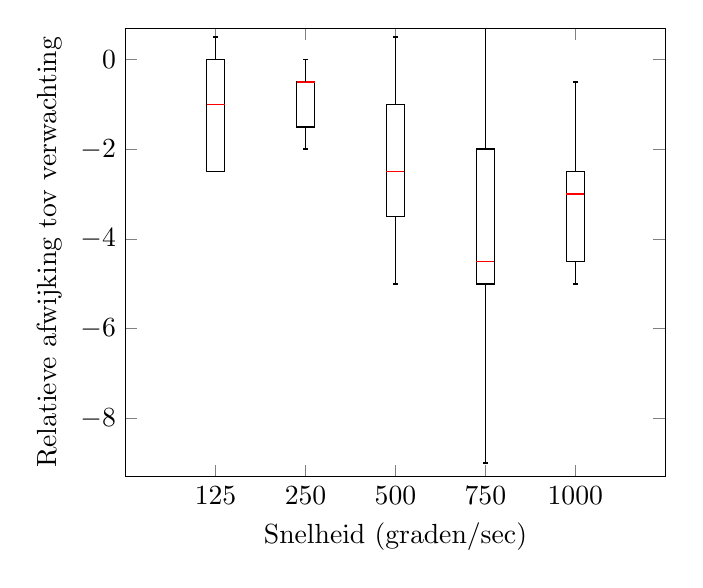
\begin{tikzpicture}
		\begin{axis}[xmin=0,xmax=6,ymin=-9.3, ymax=0.7,
			xtick={1,2,3,4,5,6},xticklabels={125,250,500,750,1000},
	      		xlabel={Snelheid (graden/sec)},
			ylabel={Relatieve afwijking tov verwachting},
			]
			%#1: center, #2: median, #3: 1/4 quartile, #4: 3/4 quartile, #5: min, #6: max
			\boxplot{1}{-1.0}{-2.5}{0}{-2.5}{0.5}
			\boxplot{2}{-0.5}{-1.5}{-0.5}{-2}{0}
			\boxplot{3}{-2.5}{-3.5}{-1.0}{-5.0}{0.5}
			\boxplot{4}{-4.5}{-5}{-2}{-9}{1.5}
			\boxplot{5}{-3.0}{-4.5}{-2.5}{-5}{-0.5}
		\end{axis}
	\end{tikzpicture}
\end{figure}

Uit de resultaten besloten we dat 250 graden per seconde ons de meest betrouwbare snelheid gaf.

Met deze snelheid werden vervolgens opnieuw verschillende afstanden gereden. De resultaten bevestigden de eerder gevonden foutmarge van ongeveer 1\%.

Dat de kwaliteit van de Lego onderdelen van groot belang kan zijn, bleek toen het omwisselen van twee wielen een oplossing bleek te zijn voor een grote afwijking naar \'e\'en bepaalde kant.

\subsubsection{Test 3: hoeken}

Het ter plekke draaien is ook gebaseerd op de wielomtrek, echter nu in combinatie met de draaicirkel die bepaald wordt door de wielafstand.

Om de nauwkeurigheid van het ter plekke draaien te bepalen, lieten we de robot 5 maal een zelfde hoek draaien. Hierbij varieerden we de hoeken als volgt: 15, 30, 45, 60 en 90 graden. Opnieuw keken we naar de eindopgave. We verwachten niet dat we met de robot veel hoeken groter dan 90 graden gaan moeten maken. Voor de veelhoek-opdracht, is dit normaal niet het geval, met een spreekwoordelijke uitzondering voor een driehoek.

Ook voor deze test wilden we de parameter snelheid in beschouwing nemen. Uit de eerste resultaten bleek snel dat een snelheid hoger dan de eerder vastgestelde 250 graden per seconde niet accepteerbare afwijkingen opleverde. Deze testen werden niet weerhouden.

De resultaten voor de verschillende hoeken zijn weergegeven in figuur \ref{chart:test3}.

\begin{figure}
	\caption{Test 3 : Relatieve afwijking bij vaste snelheid}
	\label{chart:test3}
	\vspace{10pt}	
	\centering
	
	\tikzset{external/remake next}
	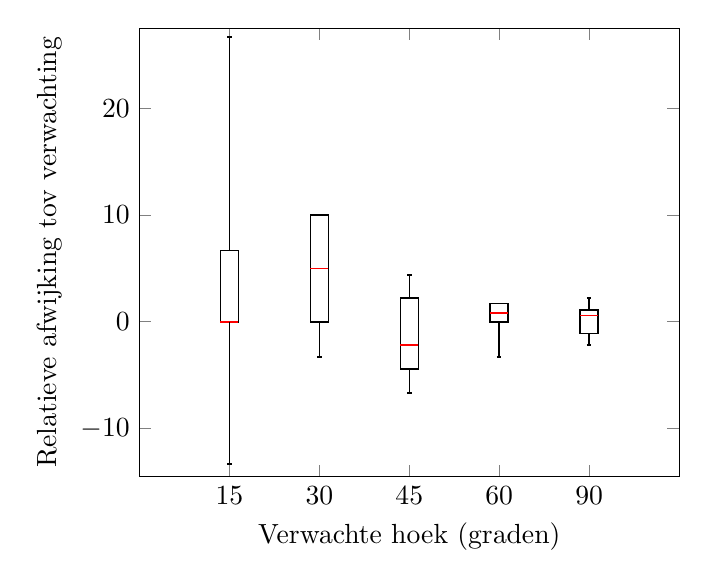
\begin{tikzpicture}
		\begin{axis}[xmin=0,xmax=6,ymin=-14.5, ymax=27.5,
			xtick={1,2,3,4,5,6},xticklabels={15,30,45,60,90},
	      		xlabel={Verwachte hoek (graden)},
			ylabel={Relatieve afwijking tov verwachting},
			]
			%#1: center, #2: median, #3: 1/4 quartile, #4: 3/4 quartile, #5: min, #6: max
			\boxplot{1}{0}{0}{6.67}{-13.3}{26.67}
			\boxplot{2}{5}{0}{10}{-3.3}{10}
			\boxplot{3}{-2.2}{-4.4}{2.2}{-6.7}{4.4}
			\boxplot{4}{0.8}{0}{1.7}{-3.3}{1.7}
			\boxplot{5}{0.6}{-1.1}{1.1}{-2.2}{2.2}
		\end{axis}
	\end{tikzpicture}
\end{figure}

De resultaten bevestigen het vermoeden dat de meetfout groter is bij kleinere hoeken. De resultaten bij 60 en 90 graden zijn dan weer positief in het kader van de einddoelstelling, waar het parcours typisch hiermee opgebouwd wordt.

\subsubsection{Conclusie ivm omwentelingen}

Met een snelheid van 250 graden per seconde en een bijstelling van de omtrek van het wiel met 1\% zou de robot, volgens onze metingen, vrij precies een willekeurige veelhoek moeten kunnen rijden.

Dit werd bevestigd bij het toepassen van deze implementatie voor het rijden van een veelhoek. Hierbij werden testen gedaan waarbij achtereenvolgens een 3, 4, 5, 6, 10 en 15-hoek werd gereden met een zijde van 20 of 30 cm. De 3, 4, 5 en 6-hoeken waren nagenoeg perfect. Bij de 10 en 15 hoek merkten we de (toen nog niet bijgewerkte) fout van 1\% op.

Figuur \ref{fig:resultsLargePolygons} toont het papier waarop we start en eindpunten aanduidden bij de grote veelhoeken en toont de afwijkingen van enkele metingen ten opzichte van het startpunt. De rode omtrek geeft de startpositie van de robot weer met het middelpunt aangegeven door het rode kruis. De zwarte kruisen zijn de middelpunten van 6 testen waarbij een 15 hoek met zijde 20 cm werd gereden.

\begin{figure}[htbp]
   \centering
   \caption{Meetresultaten voor grote veelhoeken.}
   \label{fig:resultsLargePolygons}
   \includegraphics[width=140mm]{resources/meetresultaten.png}
\end{figure}

\subsection{Tijd}

Het aansturen van de motoren op basis van tijd bleek geen valabel alternatief te zijn. De eerste resultaten gaven procentuele afwijkingen in de grootorde van 10 tot 20\%, zodat een verdere vergelijking met de resultaten voor de omwentelingen totaal overbodig werd. Deze piste werd dan ook verlaten.

\section{Resultaten van de demo en conclusies}

Tijdens de demo werd gevraagd om een veelhoek van eigen keuze te rijden. We kozen een driehoek met een zijde van 40cm. De afwijking van het startpunt bedroeg ongeveer 10cm. De tweede veelhoek die opgegeven werd was een tienhoek met een zijde van 20cm. De afwijking van het startpunt bedroeg ongeveer 30cm.

De resultaten van de demo weken sterk af van de eerder opgetekende waarden. Uit onderzoek bleek dat het vuil worden van de wielen de oorzaak was.

Figuur \ref{chart:vervuiling} toont de evolutie van de afwijking tijdens de eerste vijf veelhoeken, gereden met init\"ieel gekuiste wielen. We merken op dat in deze grootorde van gereden veelhoeken de fout sterk stijgt. Figuur \ref{chart:vervuiling2} toont de relatieve afwijking bij 5, 10, 15, 20, 25, en 30 gereden veelhoeken.

\begin{figure}
	\caption{Relatieve afwijking tgv. vervuiling wielen}
	\label{chart:vervuiling}
	\vspace{10pt}	
	\centering
	
	\tikzset{external/remake next}
	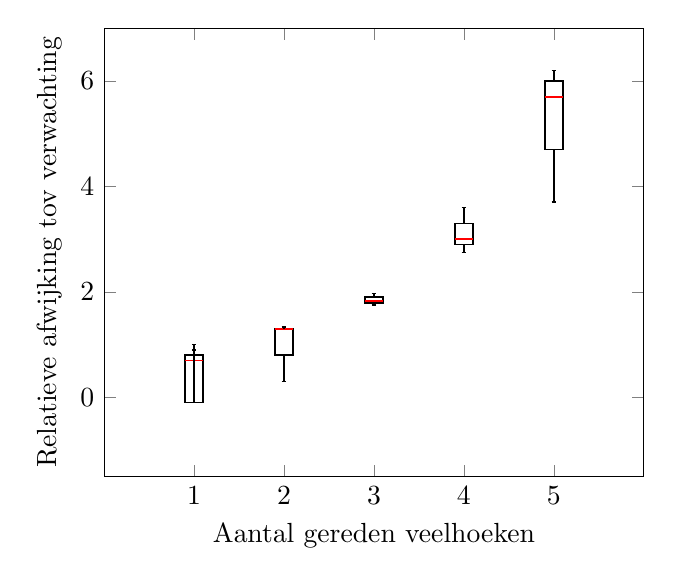
\begin{tikzpicture}
		\begin{axis}[xmin=0,xmax=6,ymin=-1.5, ymax=7,
			xtick={1,2,3,4,5,6},xticklabels={1,2,3,4,5},
	      		xlabel={Aantal gereden veelhoeken},
			ylabel={Relatieve afwijking tov verwachting},
			]
			%#1: center, #2: median, #3: 1/4 quartile, #4: 3/4 quartile, #5: min, #6: max
			\boxplot{1}{0.7}{-0.1}{0.8}{1.0}{0.9}
			\boxplot{2}{1.3}{0.8}{1.3}{0.3}{1.33}
			\boxplot{3}{1.83}{1.79}{1.9}{1.75}{1.97}
			\boxplot{4}{3.0}{2.9}{3.3}{2.75}{3.6}
			\boxplot{5}{5.7}{4.7}{6}{3.7}{6.2}
		\end{axis}
	\end{tikzpicture}
\end{figure}

\begin{figure}
	\caption{Relatieve afwijking tgv. vervuiling wielen}
	\label{chart:vervuiling2}
	\vspace{10pt}	
	\centering
	
	\tikzset{external/remake next}
	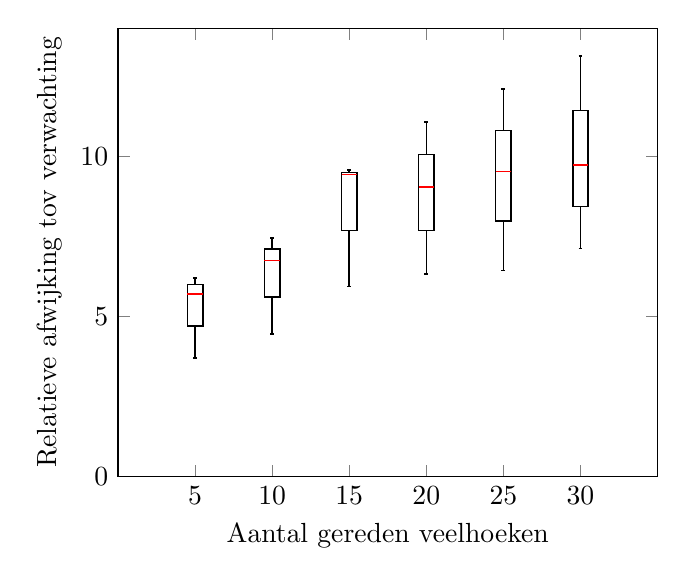
\begin{tikzpicture}
		\begin{axis}[xmin=0,xmax=7,ymin=0, ymax=14,
			xtick={1,2,3,4,5,6,7},xticklabels={5,10,15,20,25,30},
	      		xlabel={Aantal gereden veelhoeken},
			ylabel={Relatieve afwijking tov verwachting},
			]
			%#1: center, #2: median, #3: 1/4 quartile, #4: 3/4 quartile, #5: min, #6: max
			\boxplot{1}{5.7}{4.7}{6}{3.7}{6.2}
			\boxplot{2}{6.75}{5.6}{7.1}{4.45}{7.45}
			\boxplot{3}{9.43}{7.68}{9.5}{5.93}{9.57}
			\boxplot{4}{9.05}{7.69}{10.06}{6.33}{11.08}
			\boxplot{5}{9.52}{7.98}{10.81}{6.44}{12.10}
			\boxplot{6}{9.73}{8.43}{11.43}{7.12}{13.13}
		\end{axis}
	\end{tikzpicture}
\end{figure}

Uit de meting blijkt dat de fout init\"ieel sterk stijgt, maar rond 15 veelhoeken convergeert de afwijking. We zouden op basis van deze metingen kunnen besluiten dat we de robot ongeveer 15 veelhoeken zouden moeten laten rijden en vervolgens een correctie voor de gemeten fout kunnen implementeren.

Aangezien dit een specifiek probleem voor het constant rijden van veelhoeken is en dit voor de einddoelstelling geen impact heeft, implementeren we deze aanpassing niet. 

\chapter{Demo 2a: Lijnvolger}

De doelstelling van de tweede demo is het volgen van een ononderbroken lijn. Deze lijn kan wit of zwart zijn en is uitgezet op bruine panelen.

\section{Fysiek ontwerp}
\label{section:lichtsensor}

Voor het volgen van een lijn maken we gebruik van een grijswaardesensor. Deze werd vooraan op de robot bevestigd. Om de sensoren makkelijker en beter te kunnen bevestigen, werd de robot voorzien van een nieuwe structurele opbouw. Hierbij werd getracht om een zo symmetrisch mogelijk ontwerp te bekomen. Symmetrie zorgt er immers voor dat de robot zich hetzelfde gedraagt, onafhankelijk van de beweging die uitgevoerd wordt. Ook werd de wielbasis centraal geplaatst en zeer breed uitgevoerd. Dit verhoogt de laterale stabiliteit. Dubbel uitgevoerde wielen zorgen ook voor een grotere weerstand, wat nodig bleek om een helling op te geraken, ten gevolge van het gewicht van de volledige constructie.

Het nieuwe design, voorgesteld in figuur \ref{fig:redesignRobot}, voorziet tevens een opbouw waarmee een derde motor toegevoegd werd om een beweegbare sonar te realiseren. Daarnaast werden ook reeds twee druksensoren voorzien vooraan links en rechts van de robot. Deze zorgen er voor dat obstakels minder makkelijk onopgemerkt de wielen kunnen blokkeren.

\begin{figure}[htbp]
   \centering
   \caption{Redesign van het robotontwerp met alle benodigde sensoren.}
   \label{fig:redesignRobot}
   \includegraphics[width=150mm]{resources/angie.png}
\end{figure}

\section{De software}

Voor deze demo diende software ontwikkeld te worden die de robot in staat stelt om een lijn autonoom te volgen. De meetresultaten van de grijswaardesensor dienen tevens verzonden te worden via Bluetooth naar een PC, waar ze gevisualiseerd  worden. De ontwikkelingen voor robot en PC worden in dit deel verder toegelicht. De communicatie component wordt in bijlage \ref{appendix:bluetooth} in detail besproken.

\subsection{Robot}

De grijswaardesensor kan gekalibreerd worden, waarna deze genormaliseerde waarden terug geeft van 0 tot 1024\footnote{Re\"ele waarden liggen typisch tussen 145 voor een meting in een donkere omgeving en 890 in klaar zonlicht.}. Voor het kalibreren kunnen een donker- en lichtwaarde aan de Lejos API gegeven worden, welke dan gebruikt worden om de genormaliseerde waarden op af te stemmen.

Het algoritme van de robot is zeer eenvoudig gehouden, om de betrouwbaarheid te bevorderen. De volgende stappen worden in een oneindige lus uitgevoerd:

\begin{enumerate}
\item lees de genormaliseerde waarde van de grijswaardesensor
\item bepaal of de gemeten grijswaarde overeenstemt met een lijn; indien ja, rij verder rechtdoor
\item indien niet (meer) op een lijn, zoek een lijn door ter plekke heen en weer te draaien in steeds groeiende hoeken tot een lijn gevonden is
\end{enumerate}

Voor dit algoritme werd de manier waarop de Lejos API aangesproken werd gewijzigd. Voor het rijden van veelhoeken werd aan de Lejos API de opdracht gegeven om een bepaald aantal omwentelingen te doen. Vervolgens werd er gewacht om een synchrone verwerking te simuleren voor onze software. Met de introductie van sensoren en de nood om acties te ondernemen voor een bepaalde afstand bereikt is, werd deze synchrone verwerking verwijderd en zal de controle onmiddellijk teruggegeven worden aan de controleren applicatie, in dit geval het lijnvolger algoritme.

\subsection{PC}

Op de PC voorzien we een User Interface die een visuele voorstelling biedt van de door de robot opgemeten grijswaarden, gedetecteerde barcodes en bijhorende actie die ondernomen wordt. Figuur \ref{fig:demo2UI} toont de User Interface die voor de drie onderdelen van de demo zal gebruikt worden.

\begin{figure}[htbp]
   \centering
   \caption{User Interface voor Demo 2.}
   \label{fig:demo2UI}
   \includegraphics[width=150mm]{resources/demo2-ui.png}
\end{figure}

Aan de linkerkant wordt de gemeten grijswaarde weergegeven: als getal, als grijswaarde en als ge\"interpreteerde kleur (bruin, wit of zwart). Aan de rechterkant wordt een eventueel gedetecteerde barcode gevisualiseerd, als ook een indicatie van de actie die de robot zal uitvoeren op basis van deze informatie.

De User Interface bevat geen logica om enige conclusie te trekken en visualiseert louter de door de robot doorgestuurde gegevens. De robot stuurt dus de grijswaarde, de ge\"interpreteerde kleur, de barcode en actie door naar de PC.

\section{Testplan en resultaten}

Met de grijswaardesensor willen we drie kleuren kunnen onderscheiden: bruin, wit en zwart. De grijswaardesensor zal typisch verschillende waarden geven binnen een bepaald bereik voor elk van de kleuren. Het kalibreren van de lichtsensor zal bepalend zijn voor de nauwkeurigheid van deze bereiken.

We hebben met verschillende sets van kalibratiewaarden telkens 12 metingen gedaan van bruin, wit en zwart. Voor het bepalen van de waarden waarbinnen we besluiten of een kleur bruin, wit of zwart is, bekijken we de resultaten in absolute vorm over alle metingen heen. Figuur \ref{chart:kleuren} illustreert de bereiken van de drie verschillende kleuren.

Hierbij merken we op dat het bereik van de metingen voor zwart ver ligt van het bereik van bruin en wit. Deze twee laatsten daarentegen hebben wel minima en maxima die in elkaars buurt liggen en potentieel kunnen zorgen voor ``valse positieve'' in beide richtingen.

\begin{figure}
	\caption{Absolute gemeten waarden voor wit, bruin en zwart}
	\label{chart:kleuren}
	\vspace{10pt}	
	\centering
	
	\tikzset{external/remake next}
	\begin{tikzpicture}
		\begin{axis}[xmin=0,xmax=4,ymin=-15, ymax=130,
			xtick={1,2,3,4},xticklabels={wit,bruin,zwart},
	      		xlabel={Kalibratie set},
			ylabel={Gemeten grijswaarde},
			]
			%#1: center, #2: median, #3: 1/4 quartile, #4: 3/4 quartile, #5: min, #6: max
			\boxplot{1}{102}{97.25}{105}{85}{120}
			\boxplot{2}{74}{73}{76}{69}{80}
			\boxplot{3}{4.5}{-0.25}{10.25}{-10}{25}
		\end{axis}
	\end{tikzpicture}
\end{figure}

\section{Resultaten van de demo en conclusies}

De robot volgde de lijn zoals we verwachtten. Tijdens het zoeken naar een lijn werd terecht opgemerkt dat de robot te snel stopte met draaien, waardoor hoeken in te veel aparte segmenten werden afgelegd. We waren ons aan het begin van de demo bewust van dit aspect, dat toe te wijzen is aan het feit dat we niet meer tijd genomen hadden om de verschillende instelbare waarden in detail te verfijnen. 

\chapter{Demo 2b: Muurvolger}

De doelstelling van de derde demo is het volgen van een ononderbroken muur.

\section{Fysiek ontwerp}

Voor het volgen van een muur dient de sonarsensor gebruikt te worden. We hebben in ons ontwerp gekozen om de sonar te combineren met de derde motor om zo een richtbare sonar te bekomen, onafhankelijk van de ori\"entatie van de robot.

\section{De software}

Het algoritme dat we toepassen om een muur te volgen berust op het feit dat de kortste afstand tussen de robot en de muur steeds de lijn is die loodrecht op de muur staat. Het doel van de robot is om zichzelf ook loodrecht t.o.v. deze lijn te positioneren en zo evenwijdig met de muur te bewegen. Figuur \ref{fig:muurvolgerAlgoritme} illustreert dit principe.

\begin{figure}[htbp]
   \centering
   \caption{Bepalen van evenwijdige rijrichting tov een muur.}
   \label{fig:muurvolgerAlgoritme}
   \includegraphics[width=80mm]{resources/muurvolger.png}
\end{figure}

Dankzij de richtbare sonar, kan de robot zowel de afstand tot de te volgen muur meten als voor zich controleren of er geen muur is, ten gevolge van een hoek in het parcours. De robot zal de sonar dus constant heen en weer laten bewegen om deze twee punten te controleren.

De implementatie van dit principe zal gebeuren aan de hand van een aparte thread die de constante beweging van de sonar regelt en meetwaarden ter beschikking stelt van de thread die het volgen van de muur implementeert. Initieel zal een zoekroutine voorzien worden om na te gaan of er een muur links of rechts dient gevolgd te worden.

Om deze richtbare sonar initieel recht vooruit te positioneren, voorzien we een automatische calibratie op basis van een v\'o\'or de robot opgesteld obstakel. De robot zal vervolgens de kortste afstand tot dit obstakel zoeken door de sonar te laten ronddraaien en metingen te doen.

\section{Testplan en resultaten}

In tegenstelling tot het rijden en de lichtsensor, verliepen de testen voor de sonarsensor anders: de sonarsensor meet constant dezelfde waarde in gelijke omstandigheden. Ook verschil in materiaal gaf zo goed als geen afwijkingen. We bekijken vervolgens metingen met de sonarsensor in een rechthoek tot een obstakel en het effect van een hoek op de meetresultaten. Tot slot bekijken we de invloed van rijden op het meten van afstanden.

\subsection{Afstand}

In een eerste test bepaalden we de afwijking op een afstandsmeting van 1 tot 60cm. Figuur \ref{chart:sonarDistance} geeft de absolute fout weer op verschillende gemeten afstanden.

\begin{figure}[htbp]
   \centering
   \caption{Test 1: Absolute afwijking van de sonarsensor tov de te meten afstand.}
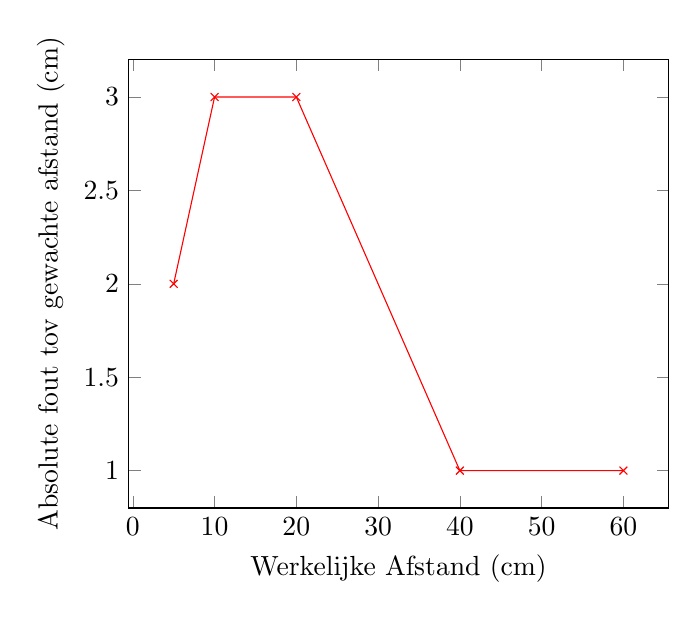
\begin{tikzpicture}
    \begin{axis}[
        xlabel=Werkelijke Afstand (cm),
        ylabel=Absolute fout tov gewachte afstand (cm)]
    \addplot[color=red,mark=x] coordinates {
	(5,2)
	(10,3)
	(20,3)
	(40,1)
	(60,1)
   };
    \end{axis}
\end{tikzpicture}
   \label{chart:sonarDistance}
\end{figure}

Hierbij valt onmiddellijk op dat de sonar beduidend correcter meet op grotere afstand en een grotere fout laat optekenen bij kleinere.

\subsection{Hoek}

Een robot zal niet steeds loodrecht staan t.o.v. een obstakel. Het principe van de sonarsensor berust op weerkaatsing van uitgezonden golven. Vanaf een hoek van 45 graden, zullen deze golven niet meer teruggekaatst worden. Elementaire testen toonden dit aan.

\subsection{Rijden}

De robot zal hoofdzakelijk metingen doen terwijl hij rijdt. Het is daarom interessant om te weten of dit een grote impact heeft. Een test werd gedaan waarbij de robot op een afstand van een obstakel werd geplaatst en naar het obstakel toe reed. Hierbij registreerde de robot informatie van de tachometer en van de sonarsensor. Op basis van deze gegevens kunnen we de metingen van de sonar afstemmen op de afstand berekend door de tachometer. We hebben een 15-tal metingen voor deze test gedaan en de meetresultaten waren telkens ongeveer identiek. Ze vertoonden ook een typisch patroon, zoals weergegeven in figuur \ref{chart:sonarDrive}.

\begin{figure}[htbp]
   \centering
   \caption{Test 3: Absolute fout van de sonarsensor bij rijdende meting.}
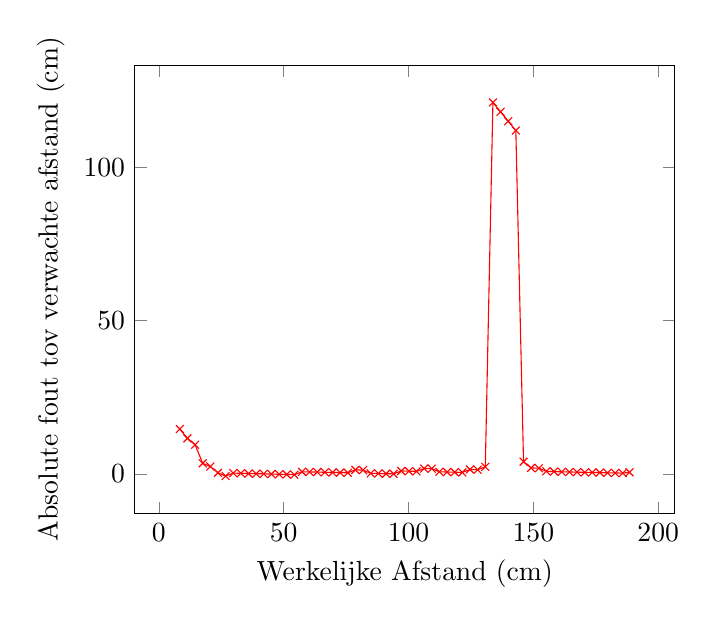
\begin{tikzpicture}
    \begin{axis}[
        xlabel=Werkelijke Afstand (cm),
        ylabel=Absolute fout tov verwachte afstand (cm),
       legend style={draw=none}]
    \addplot[color=red,mark=x,] coordinates {
(188.50,0.50)
(185.78,0.22)
(182.73,0.27)
(179.68,0.32)
(176.60,0.40)
(173.55,0.45)
(170.54,0.46)
(167.46,0.54)
(164.41,0.59)
(161.36,0.64)
(158.28,0.72)
(155.18,0.82)
(152.18,1.82)
(149.08,1.92)
(146.05,3.95)
(142.97,112.03)
(139.92,115.08)
(136.84,118.16)
(133.79,121.21)
(130.74,2.26)
(127.66,1.34)
(124.58,1.42)
(121.55,0.45)
(118.48,0.52)
(115.42,0.58)
(112.35,0.65)
(109.32,1.68)
(106.27,1.73)
(103.19,0.81)
(100.16,0.84)
(97.08,0.92)
(94.01,-0.01)
(90.98,0.02)
(87.90,0.10)
(84.85,0.15)
(81.80,1.20)
(78.72,1.28)
(75.67,0.33)
(72.61,0.39)
(69.56,0.44)
(66.51,0.49)
(63.43,0.57)
(60.40,0.60)
(57.35,0.65)
(54.30,-0.30)
(51.20,-0.20)
(48.15,-0.15)
(45.09,-0.09)
(42.02,-0.02)
(38.96,0.04)
(35.93,0.07)
(32.83,0.17)
(29.78,0.22)
(26.73,-0.73)
(23.68,0.32)
(20.62,2.38)
(17.57,3.43)
(14.52,9.48)
(11.44,11.56)
(8.41,14.59)
   };
    \end{axis}
\end{tikzpicture}
   \label{chart:sonarDrive}
\end{figure}

De robot vertrok op 180cm van het obstakel. Zoals we reeds opmerkten in de voorgaande testen, is de sonar relatief nauwkeurig op grotere afstanden. Vanaf 30cm vergroot de fout aanzienlijk.

Er is een piek die zich voordoet rond de 130 tot 140cm. Op deze afstand detecteert de sensor geen obstakels. We vermoeden dat er zich hier een eigenfrequentie optreedt en dat er golffronten samenvallen. Dit heeft waarschijnlijk te maken met de manier waarop de sonar fysiek werkt. Aangezien we voor de doelstellingen van de verschillende demo's geen informatie nodig hebben voor afstanden boven de 80cm, is dit fenomeen onbelangrijk voor ons. Deze observatie werd door andere groepen bevestigd.

De meetwaarden van deze test waren omvangrijk in aantal. Ze werden dan ook met behulp van de Bluetooth verbinding doorgestuurd naar de PC voor verdere verwerking in een spreadsheet.

\section{Resultaten van de demo en conclusies}

De robot was in staat om meerdere rondjes op het parcours te rijden. Het algoritme voorzag een robot die vooruitreed en veranderen slechts van richting op basis van een nieuwe volledige set van sonar-waarden. De tijd om een volledige ``sweep'' uit te voeren was echter soms te lang om tijdig van richting te veranderen om een obstakel te vermijden. Naar de finale demo toe willen we de verhouding tussen het rijden en het detecteren van obstakels met de sonar, verder verfijnen.

\chapter{Demo 2c: Barcode}

De doelstelling van de vierde demo is het detecteren van barcodes op een eenvoudig parcours. Op basis van de informatie die deze barcodes aanbieden moet de robot zijn weg vinden naar de volgende barcode en zo het parcours 1 keer afleggen.

\section{Fysiek ontwerp}

Voor het lezen van barcodes gebruiken we de grijswaardesensor. Deze is reeds op de robot gemonteerd, zoals besproken in sectie \ref{section:lichtsensor}. Eveneens de basissoftware om grijswaarden te registeren wordt opnieuw gebruikt.

\section{De software}

Het algoritme dat op basis van de gemeten grijswaarden barcodes doorloopt een oneindige lus, waarin steeds een genormaliseerde waarde van de grijdwaardesensor gelezen wordt. Op basis van de calibratiewaarden wordt deze waarde omgezet in een kleur: bruin, wit of zwart.

Algemeen kent het algoritme twee grote statussen:

\begin{enumerate}
\item Gewoon rijden, op zoek naar een barcode.
\item Een gevonden barcode bepalen.
\end{enumerate}

Bij het zoeken naar een barcode worden bruine metingen genegeerd. Niet-bruine waarden brengt het algoritme in een status waarbij de gevonden barcode bepaald wordt. In die status worden alle niet-bruine waarden bewaard tot er opnieuw 5 bruinwaarden opgemeten zijn. Indien er minstens 3 niet-bruine waarden opgemeten zijn, wordt een barcode bepaald.

Hiervoor worden de opgemeten waardes in 7 gelijke groepen verdeeld. Voor elk van deze groepen wordt het gemiddelde bepaald en vertaald naar wit of zwart. Deze 7 wit/zwart waarden kunnen vertaald worden naar een reeks van 1-en en 0-en, welke ge\"interpreteerd worden als een getal.

Tot slot wordt aan de hand van een tabel de effectief gedetecteerde waarde omgezet naar een gecorrigeerde waarde volgens de Hamming-code error-correctie.

\section{Testplan en resultaten}

De verschillende barcodes werden meermaals door de robot gedetecteerd, zowel recht-rijdend als onder verschillende hoeken. Alle testen resulteerden in een correct gelezen barcode.

\section{Resultaten van de demo en conclusies}

De robot detecteerde de barcodes correct, behalve de barcodes die zich op een helling bevonden. Om dit probleem op te lossen moeten we het fysieke ontwerp van de robot verder verfijnen, zodat de hoek van de helling geen negatieve impact heeft op de positie van de grijswaardesensor.

\chapter{Finale demonstratie}

Tijdens de finale demonstratie moet de robot autonoom een onbekend parcours rijden. Hierbij kan gebruik gemaakt worden van alle sensoren. Op het parcours kunnen panelen voorkomen waar maximaal \'e\'en met een sensor waarneembare eigenschap weggenomen wordt.

\section{Fysiek ontwerp}

Het fysieke ontwerp van de robot is ongewijzigd gebleven sinds de vorige demo. We hadden tijdens die iteratie reeds de geplande aanpassingen gedaan. Een poging om een betere bevestiging van de lichtsensor te bekomen op basis van een parallellogram leverde geen noemenswaardige verbeteringen op. Met het oog op het rijden van een parcours beschouwen we het falen om een barcode te lezen als een eigenschap waar de robot bestand moet tegen zijn.

\section{De software}

Na de tussentijdse demo's zijn we voor het rijden van het parcours overgeschakeld op onze langere termijn strategie. Hiervoor werd een simulatieomgeving ontworpen om onafhankelijk van de fysieke robot te kunnen testen en experimenteren. We belichten de simulator kort, vooraleer we het eigenlijke huidige algoritme bespreken. Daarna bekijken we tevens kort het nieuwe logging framework en de nieuwe web-interface.

\subsection{Simulator}

Het ontwikkelen van software voor een door Lejos aangedreven Mindstorms robot, of eender welk ander ``embedded'' systeem, wordt typisch bemoeilijkt door de zeer beperkte toegankelijkheid van het systeem. Deze ontoegankelijkheid vertoont zich op verschillende vlakken: op fysiek vlak dient er steeds een nieuwe versie van de software overgebracht worden, moet de robot op een parcours geplaatst worden (dat eerst nog gebouwd moet worden), enz. Op vlak van software ontwikkeling is men niet in staat om normale ontwikkelomgevingen te gebruiken en kan nauwelijks of met grote omwegen ``gedebugged'' worden.

We hebben daarom gekozen om een simulatieomgeving te cre\"eren waar we zelf alle controle over hebben en die de bovengenoemde problemen grotendeels oplost. Figuur \ref{fig:simulator} toont de simulator in actie.

\begin{figure}[htbp]
   \centering
   \caption{Simulator in actie.}
   \label{fig:simulator}
   \includegraphics[width=150mm]{resources/simulator.png}
\end{figure}

De simulator stelt ons in staat om de exacte code die uiteindelijk op de robot zal gebruikt worden uit te voeren. Hierbij zal de simulatieomgeving de invoer voor de sensoren berekenen op basis van een voor-gedefinieerd parcours. De acties van de robot, uitgedrukt in veranderingen van de motoren, worden ook door de simulatieomgeving opgepikt en vervolgens omgezet in realistische verplaatsingen op het parcours.

Het is belangrijk de simulator niet hoofdzakelijk te bekijken als een volledig alternatief voor een fysieke robot. De simulator bewijst in de eerste plaats zijn nut als een software development tool. Het is altijd mogelijk om te controleren of een algoritme juist werkt, door te kijken of de robot in gesimuleerde situatie correct reageert. 

Andere voordelen van de simulator zijn:
\begin{enumerate}
\item korte iteratietijden bij aanpassingen aan de code
\item determinisme van de sensoren en de motoren, dit vereenvoudigt het testen
\item sneller dan real-time simulatie van de robot spaart veel tijd uit
\item eenvoudige localisatie van exceptions; doordat alle code reeds uitgevoerd is op de PC, komen er geen exceptions meer voor op de robot
\end{enumerate}

Meermaals heeft de Simulator zijn nut bewezen. Verschillende teamleden hebben in parallel kunnen werken aan verschillende Navigatoren. De volledige logica van de Robot is bvb. ontwikkeld binnen de Simulator. Bij het overzetten naar de fysieke robot dienden slechts enkele parameters met betrekking tot de synchronisatie van de verschillende threads proefondervindelijk bijgewerkt te worden. In beide omgevingen werkt het algoritme principieel op de zelfde manier.

Bijlage \ref{appendix:simulator} belicht de simulator in groter detail en verklaart enkele van de design-keuzes die we genomen hebben, wat de gevolgen er van waren en hoe deze pasten in de gekozen strategie.

\subsection{Model, ModelProcessoren en Navigator}

De centrale logica van de robot is opgebouwd uit verschillende componenten. Alle informatie die opgetekend wordt van de sensoren wordt opgeslagen in een centraal \texttt{Model}. Op dit Model werken verschillende onafhankelijke \texttt{ModelProcessoren} om de ruwe data om te vormen tot informatie. Tot slot zal een \texttt{Navigator} op basis van alle informatie in het Model een beslissing nemen.

De drie componenten, Model, ModelProcessoren en Navigator bepalen de Robot en kunnen onafhankelijk van elkaar geoptimaliseerd worden. We hebben op die manier \'e\'en Model ontwikkeld, een groot aantal ModelProcessoren en verschillende Navigatoren. Elk van de tussentijdse demo's hebben we zo ook ge\"implementeerd als Navigator.

Een voorbeeld van een ModelProcessor is de HistogramModelProcessor. Deze zorgt er voor dat het model een histogram bevat van de grijswaarden. Andere ModelProcessoren kunnen deze uitgebreidere informatie dan weer gebruiken om barcodes of lijnen te detecteren.

Al deze componenten werken zonder enige wijzigingen zowel op de fysieke robot als in de Simulator, dankzij de abstractie op nieuw van de RobotAPI.

Details omtrent het Model, de Modelprocessoren en de Navigator kunnen teruggevonden worden in bijlage \ref{appendix:classDiagrams}, met klasse diagrammen voor deze componenten.

\subsection{Algoritme}

Oorspronkelijk hadden we het plan opgevat om in het Model een virtuele map op te bouwen en deze te gebruiken bij het navigeren. Dit zou in theorie een interessante bron van informatie geweest zijn bij het rijden van een tweede ronde op een zelfde parcours.

We zijn van dit plan afgestapt omdat deze soort informatie eigenlijk een zeer precieze robot vereist, die in staat is om zijn positie redelijk nauwkeurig te bepalen op basis van de informatie van zijn sensoren. Dit is een veel te strenge eis vergeleken met de doelstelling om een robuuste robot te ontwerpen.

We hebben onze strategie aangepast en er voor gekozen om de robot zo te ontwerpen dat hij op elk ogenblik onafhankelijk van voorgaande situaties zijn volgende actie bepaalt. Dit resulteert in een robot die zelfs een onlogische verandering aankan. We denken hierbij bvb. aan botsingen met andere robots, extreme verschuivingen tgv. vuile wielen en/of schuine parcours, enz.

De uitwerking van het algoritme zelf ziet er uit als volgt:

\begin{enumerate}
\item detecteren van events uit de wereld
\item uitvoeren van acties die zich op de \texttt{ActionQueue} bevinden.
\end{enumerate}

Tijdens het detecteren van de events uit de wereld, bekijkt de Navigator de volgende mogelijke gebeurtenissen in volgorde:

\begin{enumerate}
\item nabijheid van obstakels
\item detectie van barcodes
\item detectie van lijnen
\item botsing situaties
\end{enumerate}

Indien \'e\'en van deze gebeurtenissen voorvalt, zal de Navigator de nodige acties op de \texttt{ActionQueue} plaatsen. Dit is een queue van acties die ondernomen moeten worden. Bij een botsing zal er bvb. eerst achteruit gereden worden en vervolgens gedraaid worden.

De volgende acties staan ter beschikking van de Navigator:

\begin{itemize}
\item MoveAction: de robot rijdt een bepaalde afstand
\item TurnAction: de robot draait een bepaalde hoek
\item StopAction: de robot onderbreekt de huidige actie
\item DriveForwardAction: de robot rijdt vooruit, zonder beperking in afstand
\item MoveOffLineAction: de robot draait tot zijn lichtsensor terug aan de andere kant van de lijn is
\end{itemize}

Bijlage \ref{model:actions} bevat een klasse diagram waarin alle acties in detail weergegeven worden.

Elk van deze acties kan tot slot in een niet-onderbreekbare staat gebracht worden, waardoor deze niet onderbroken worden wanneer er andere events gedetecteerd worden.

Indien de robot geen acties meer in zijn queue heeft, gaat hij ``gap detection'' gebruiken om zijn richting te bepalen. Wanneer de robot uit sonarmetingen kan vaststellen dat hij in alle richtingen zal botsen, behalve in 1 duidelijk begrensde richting, ``the gap'', dan zal de robot zich richten naar die gap. Dit algoritme bleek zeer krachtig. In een volledig door muren begrensd parcours is gap detection voldoende om een zeer goed rij-resultaat op te leveren.

Als er uit alle voorgaande condities niets besloten kon worden, rijdt de robot gewoon vooruit.

\subsection{Logging en Web-interface}

Naast de overschakeling naar de model-gedreven navigator, is ook de manier van het verwerken van feedback van de robot gewijzigd. De robot zendt nu de informatie uit het model en de navigator door naar de PC. Deze gegevens worden nu niet langer rechtstreeks getoond in een grafische gebruikersinterface, maar worden via het log4j logging framework zo snel mogelijk in een relationele databank opgeslagen. Aan de hand van een REST-ful web-service, aangeboden van op een JBoss applicatie server, wordt nu de informatie weergegeven op een HTML/CSS/Javascript-gebaseerde interface. Figuur \ref{fig:webclient} toont de nieuwe web interface.

\begin{figure}[htbp]
   \centering
   \caption{De nieuwe webclient.}
   \label{fig:webclient}
   \includegraphics[width=150mm]{resources/webclient.png}
\end{figure}

De webinterface tracht een getrouw beeld te geven van de informatie die zich op een bepaald moment in de software op de robot bevindt. Zo wordt het model en de navigator onafhankelijk voorgesteld. Binnen het model worden de verschillende sensoren weergegeven met hun gemeten waarden, alsook de interpretatie ervan. De histogrammen van de licht- en sonarsensoren, die in het model van de robot worden opgebouwd worden in de interface gevisualiseerd als een echt visueel histogram en een vlakafbakening die aangeeft welke ruimte de robot voor zich als``vrij'' beschouwd.

De webinterface biedt ook de mogelijkheid om de stroom die van de applicatieserver komt te pauzeren en stapsgewijs verder te zetten. Deze eenvoudige debug-mogelijkheden hebben ons tijdens de laatste voorbereidingen enorm geholpen om volledig te begrijpen wat de robot ``zag'' en zo ook beter wat de bijhorende beslissingen veroorzaakte.

Bijlage \ref{appendix:ui} beschrijft meer aspecten van de user interface alsook de functionaliteit en mogelijkheden.

\section{Resultaten van de demo en conclusies}

Onze doelstelling om een robuuste robot te ontwikkelen was een succes. Dit bleek tijdens de finale demo. De opstelling van het finale parcours bevatten verschillende uitzonderlijke configuraties van panelen die zowel de fysieke design van de robot als de software enorm op de proef stelden. Onze robot wist elk van deze speciale opstellingen te overwinnen, hetzij door zijn fysieke eigenschappen (zoals bvb de positie van de wielen), het zij door de software (bvb door het positieve gebruik van de sonar om een goede richting te kiezen), hetzij door een combinatie van de twee waarbij de werking van de software en de fysieke eigenschappen samen een oplossing boden (bvb door frontale druksensoren, een ontwijkingsalgoritme en een brede wielbasis).

Op twee plaatsen in het parcours las de robot echter een verkeerde barcode, waardoor een bocht naar links naar rechts werd ingezet. Ook een daaropvolgende zwarte lijn werd niet herkend. We hebben dezelfde situatie proberen te reconstrueren, echter zonder succes. We moeten concluderen dat de calibratie van de grijswaardensensor niet optimaal was voor die specifieke situatie.

Het kalibreren van de grijswaardensensor is eigenlijk nog het enige externe aspect van de robot dat een variatie kan geven in het gedrag van de robot. We hebben ge\"experimenteerd met een manier waarbij dit overbodig wordt. Hierbij worden de twee ``thresholds'' op basis van alle gelezen waarden steeds bijgewerkt, waardoor er een evoluerende begrip van de grijswaarden optreedt. Dit kan helpen om wisselende belichtingsomstandigheden op te vangen. We hebben dit algoritme echter niet meer last-minute durven opnemen in de uiteindelijk configuratie voor de finale demo. Mogelijk is dit echter wel een antwoord op het probleem dat waarschijnlijk aan de oorsprong lag van de dubbele fout, namelijk de verkeerd ge\"interpreteerde barcode en onopgemerkte zwarte lijn, die zich voordeed tijdens de demo.

Wat betreft verdere optimalisaties zouden we op basis van dit resultaat vooral kijken naar een verhoging van de basissnelheid of de mogelijkheid om de snelheid te laten vari\"eren in functie van rechtdoor rijden of het nemen van bochten.

Met de huidige softwaresetup, liepen we stilaan tegen de limieten van de robot. Bepaalde situaties resulteerden duidelijk in een vertraging van de event loop, waardoor soms niet voldoende metingen konden gedaan worden door de sensoren. We hebben voor de finale demo een goed evenwicht gevonden tussen snelheid van de robot en complexiteit van de verwerking. We zijn van mening dat we door het verbeteren van de algoritmes en het effici\"enter omspringen met CPU cycli, we de ``frame rate'' van de event loop nog sterk kunnen doen stijgen, waardoor de frequentie van de metingen drastisch kan verhoogd worden, waardoor we in staat zijn om de snelheid van de robot te verhogen.

\chapter{Het proces}

D\'e uitdaging in dit groepswerk was de robot. Niet zozeer de technische aspecten, maar wel het feit dat er maar \'e\'en robot ter beschikking van elk team stond. Hierdoor was een goede organisatie en planning van het werk soms niet eenvoudig. Dit gecombineerd met een strak tijdschema waarbinnen de twee eerste tussentijdse demo's dienden opgeleverd te worden.

Deze reden alleen was reeds voldoende om de ontwikkeling van een simulatieomgeving te verantwoorden. Maar deze aanpak was ook van cruciaal belang omdat we geconfronteerd werden met een zeer ontoegankelijke ``embedded'' omgeving. Dankzij de simulatieomgeving waren we in staat om verschillende aspecten van onze architectuur uit te testen en vorm te geven in een omgeving die ons alle mogelijkheden biedt die normaal beschikbaar zijn.

We opteerden ook heel expliciet om twee afzonderlijke trajecten te volgen: een eerste volgde de verplichte tussentijdse demo's, terwijl een tweede traject focuste op de finale demo. Hierbij werd een architectuur uitgetekend die een robuuste robot nastreefde, maar die overbodig was voor de tussentijdse evaluaties. De ontwikkeling ervan zou ook niet mogelijk zijn binnen het tijdsbestek gegeven voor de tussentijdse demo's. Deze tactiek was succesvol, maar hield ook een risico in. Vanuit ons tactisch oogpunt waren de tussentijds demo's een belasting die op zich geen toegevoegde waarde had naar de einddoelstellingen. Praktisch hebben we hier manuren moeten investeren die we niet hebben kunnen toewijzen aan het ontwikkelen van de simulator of de model/navigator architectuur. Zelf hadden we andere tussentijdse doelen voorgesteld (zoals bijvoorbeeld het bouwen van de simulator), die ons interessantere inzichten hadden kunnen verschaffen met het oog op het einddoel.

Naast de vijf uren op maandag, spendeerden we gemiddeld nog een zevental uren tijdens het verdere verloop van de week. Hierbij werden typisch twee bijkomende ogenblikken afgesproken waarop teamleden konden samenkomen om in groep te werken. Op die manier had iedereen minstens twee contactmomenten per week. Deze werden aangevuld met bijkomend werk van thuis uit. Het opsplitsen van het team in twee groepen zorgde er ook voor dat de robot optimaler te beschikking stond van alle teamleden. Deze manier van werken, een vast aantal uren en een vrij te kiezen aantal uren werd door alle teamleden positief onthaald en was zeer productief.

Tijdens de eerste sessie werden concrete afspraken gemaakt omtrent het gebruik van een versie-beheersysteem, in casu Git\footnote{http://git-scm.com}, en een centrale source code hosting, GitHub\footnote{http://github.com}. Daarnaast werd gekozen voor Google Docs\footnote{http://docs.google.com} om interne documenten, ontwerpen en spreadsheets te beheren.

Met meerdere teamleden die actief werken op een zelfde codebase, is het belangrijk om goede afspraken te maken en de code stijl te verzorgen. Ook deze aspecten werden meermaals besproken en benadrukt, waardoor er geen noemenswaardige problemen ontstonden op dit vlak. De werkwijze die door Git aangeboden wordt, werkt zeer goed en helpt elk teamlid om op een team-vriendelijke manier zijn code bij te dragen.

Ondanks de grote verschillen in achtergrond van de teamleden, was er duidelijk een vrij homogene verdeling van de kennis nodig om een project van deze omvang aan te pakken. Elk teamlid kon zijn expertise op de voorgrond laten treden en iedereen was in staat om elk aspect van de ontwikkeling te volgen.

\chapter{Werkverdeling}

\begin{longtable}{l l}
\caption{Focus van elk team lid} \\ [0.5ex]
%This is the header for the first page of the table...
\hline\hline
Teamlid & Focus \\ [0.5ex]
\hline 
\endfirsthead
%This is the header for the remaining page(s) of the table...
\multicolumn{2}{c}{{\tablename} \thetable{} -- Vervolg} \\[0.5ex]
\hline \hline
Teamlid & Focus \\ [0.5ex]
\hline 
\endhead
Michiel 		& 	(Coordinator) Bluetooth communicatie, calibratie, finale navigator. \\
Florian 		&	RobotAPI, lijnvolger, opvolgen unit testen, finale navigator. \\
Ruben 		&	RobotAPI, veelhoek algoritme, muurvolger, sonar-navigator.\\
Thomas 		&	RobotAPI, lichtsensor, barcode-lezer, fat client. \\
Daniel 		&	Testen, barcode-lezer, fat client. \\
Christophe 	&	(Secretaris) Verslag, simulator, model \& navigator, web-client. \\
\hline
\label{tab:focus}
\end{longtable}

\begin{longtable}{l r r r r r r r}
\caption{Tijdsbesteding per team lid per week} \\
%This is the header for the first page of the table...
\hline\hline
  & michiel & florian & ruben & thomas & daniel & christophe & totaal \\
\hline 
\endfirsthead
totaal & 143 & 104 & 109 & 107 & 101 & 143 & 707 \\
\hline
week 1 & 10 & 10 & 10 & 10 & 10 & 15 & 65 \\
week 2 & 9 & 7 & 8 & 7 & 9 & 16 & 56 \\
week 3 & 8 & 8 & 8 & 8 & 5 & 12 & 49 \\
week 4 & 9 & 7 & 5 & 8 & 5 & 17 & 51 \\
week 5 & 33 & 15 & 18 & 6 & 15 & 34 & 121 \\
week 6  & 15 & 11 & 12 & 18 & 15 & 5 & 76 \\
week 7 & 6 & 11 & 10 & 9 & 9 & 9 & 54 \\
week 8 & 10 & 9 & 12 & 15 & 5 & 9 & 60 \\
week 9 & 34 & 21 & 17 & 21 & 13 & 11 & 117 \\
week 10 & 9 & 5 & 9 & 5 & 15 & 15 & 58 \\
\hline
gemid./week & 14 & 10 & 11 & 11 & 10 & 14 & 12 \\
\label{tab:tijdsregistratie}
\end{longtable}

\chapter{Analyse}

Het team had zich een duidelijke doelstelling voorgesteld: een robuuste robot maken. Aan het einde van dit project zijn alle teamleden het unaniem eens dat we in die opzet geslaagd zijn. We kunnen de robot op dit ogenblik geen realistisch parcours aanbieden waar hij niet door zal geraken. Deze robuustheid gaat wel ten koste van de snelheid. Dit is een eigenschap van het ontwerp van zowel de fysieke robot als de software, maar is volledig volgens het door het team vooropgestelde  plan.

Naast de verplichte aspecten van het project, hebben we getracht om ook in een ruimer kader onze persoonlijke horizonten te verbreden. Hierbij hebben we gekeken naar de professionele realiteit en daar inspiratie opgedaan om een robuuste context te bouwen rond de robot. Zo maakten we soms misschien niet evidente keuzes, zoals een service-geori\"enteeerde architectuur voor de user interface of een iets uitgewerktere architectuur met een Model, Modelprocessoren en een Navigator. Het toevoegen van elk van deze complexiteiten bracht een risico met zich mee, maar we hebben uiteindelijk meer dan verwacht voordeel gehaald uit onze aanpak.

De resultaten van onze keuzes zijn zeker positief, maar algemeen blijven we met het gevoel achter dat alles niet af is. We hebben veel domeinen aangeraakt en er net genoeg van kunnen realiseren voor de demo's, maar de mogelijkheden van elk van de componenten zijn niet ten volle uitgediept. De simulator is bvb. al waarheidsgetrouw genoeg voor het voorbereiden van de demo's, maar bevat deze geen noties van versmallingen, hellingen, enz. Het toevoegen van deze aspecten, zou ons in staat stellen om bvb het finale demoparcours in detail te analyseren.

Waar we oorspronkelijk gedacht hadden aan een Model waarin een virtuele map van de wereld zou worden opgebouwd, zijn we van dit plan afgestapt. Het resultaat was een zeer robuuste robot, maar ook hier hadden we toch graag onderzocht hoe een ``geheugen'' onze robot nog beter had kunnen maken ... of niet.

Ook het fysieke ontwerp van de robot is zeker positief aspect aan het resultaat, maar het is slechts een tweede generatie ontwerp. Met de huidige kennis zouden we zeker bepaalde aspecten aan het ontwerp veranderen, om bepaalde fysieke aspecten van het parcours eenvoudiger op te vangen op dit niveau. Daar waar dit op dit ogenblik wel een mooi samenspel is van de software en de fysieke robot, moeten we toegeven dat dit eerder balanceert op het randje van een ``gelukkig'' samengaan van deze aspecten dan van een berekend gevolg.

De ervaring na het ontwikkelen van twee verschillende user interfaces bevestigde het gevoel omtrent de verdeling van het werk: we hebben initieel te veel de nadruk gelegd op de realisatie van de tussentijdse demo's. De tijd die in sommige aspecten van de voorbereiding hiervan is gekropen woog niet op tegen de winst die we er uitgehaald hebben. In het geval van de user interface werd meer dan 12 uur gespendeerd om een ``fat client'' te ontwikkelen. De web client die we uiteindelijk gebruikt hebben tijdens de finale demo heeft slechts 6 uur gekost, inclusief de ontwikkeling van de robot agent, het opzetten van de databank en het ontwikkelen van de REST-interface. Omdat we schrik hadden dat onze langetermijnvisie misschien niet tijdig klaar ging zijn, hebben we veel aspecten hiervan naar achter geschoven. Hadden we hier wel prioriteit aan gegeven, en meer teamleden er aan laten werken, hadden zaken zoals de web client zeker al klaar geweest voor de tweede demo en hadden we kostbare tijd gewonnen door het niet ontwikkelen van de fat client. Deze tijd hadden we dan weer kunnen spenderen aan het ontwikkelen van meer functionaliteit voor de web client, enz.

\appendix

\chapter{Software}
\label{appendix:software}

\section{Bluetooth}
\label{appendix:bluetooth}

De bluetoothlaag is opgebouwd als een volledige abstractielaag voor packetgebaseerde communicatie. Pakketten worden verstuurd tussen zogenaamde \texttt{PacketTransporter} objecten op de pc en de robot. De werkelijke connectie wordt abstract gemaakt d.m.v. de \texttt{IConnection} interface.

Deze communicatielaag realiseert de volgende technische aspecten:
\begin{itemize}
\item thread safe: PacketTransporters kunnen op verschillende threads gebruikt worden, en alle methodes zijn thread-safe.
\item pakket-queue: pakketten kunnen synchroon en asynchroon ontvangen worden, nog niet uitgelezen pakketten worden opgeslagen in een queue
\item onafhankelijkheid: elke PacketTransporter is volledig onafhankelijk van andere transporters. Een nieuwe component in de applicatie kan pakketcommunicatie toevoegen zonder dat de rest van de applicatie be\"invloed wordt.
\item robuustheid: problemen in de communicatie worden afgehandeld door de communicatielaag en hebben geen invloed op de rest van de applicatie.
\item connectie abstractie: doordat de PacketTransporters werken m.b.v. een abstracte IConnection interface, kan dezelfde code gebruikt worden met bluetooth, usb en zelfs gesimuleerde connecties.
\end{itemize}

Door een volledige abstractielaag te maken, was het niet nodig aanpassingen te maken aan de communicatie code doorheen het project. Dit kwam ten goede van de stabiliteit van deze code. De algemene implementatie van de laag geeft ook een zekere vrijheid qua gebruik. Zo kan de communicatie gebeuren op de manier die het eenvoudigst is in een bepaalde situatie.

Praktisch bestaat een packet uit een uniek 4-byte geheel getal (packettype), een stuk binaire data (dgram) en de lengte van het dgram. Communicatie gebeurt d.m.v. een PacketTransporter, die verantwoordelijk is voor het verzenden en ontvangen van packets. De PacketTransporter vormt op deze manier een virtuele connectie, die toelaat onafhankelijk informatie uit te wisselen tussen verschillende delen van verschillende programma's. De transporters ontvangen pakketen van een bepaald type, door zich te registeren bij een IConnection. Het is mogelijk om een transporter verschillende soorten pakketten te laten ontvangen.

\section{Functionaliteit}

De functionaliteit van de robot zelf is zeer beperkt gehouden. De doelstelling was een zeer robuuste robot te ontwerpen. D\'e manier om dit te bewerkstelligen is net het beperken van de complexiteit en de onderlinge afhankelijkheden tussen de verschillende componenten. We hebben getracht functionaliteit te cre\"eren rond de robot.

We hebben bvb. gekozen voor het introduceren van een robot agent die op de PC niets meer doet dat het ontvangen van informatie van de robot. Vervolgens wordt deze in een databank opgeslagen. In zijn huidige vorm is dit slechts een eenvoudig uitgewerkt opslagmedium, maar mits verdere ontwikkeling kunnen hier interessante bijkomende voordelen uit gehaald worden. De gegevens in de databank kunnen bvb. verrijkt worden met informatie over de effectieve positie van de robot (via externe positiebepaling). Al deze gegevens kunnen bijvoorbeeld opnieuw in de simulator gevoed worden waar detailanalyse mogelijk wordt. Ook zouden meerdere sessie van meerdere robots kunnen opgeslagen worden, enz.

Zelfs zonder al deze mogelijke toekomstige uitbreidingen, biedt het huidige platform reeds de mogelijkheid om met verschillende browsers een stroom van de robot te visualiseren, te pauzeren, stap voor stap te bekijken, enz.

Het ontwikkelen van ``embedded software'' is op zich geen sinecure. De robot is verre van een toegankelijke omgeving en het debuggen van software ervoor wordt sterk bemoeilijkt door de beperkingen van de robot en zijn OS. De simulator biedt echter een omgeving waarin we bevrijd worden van de meeste van deze beperkingen en liet ons toe om in een normale omgeving de belangrijkste aspecten van de robot te ontwikkelen.

\section{Klasse Diagrammen}
\label{appendix:classDiagrams}

In deze bijlage verzamelen we verschillende klasse diagrammen die samen een concreet overzicht geven van de ontwikkelde software. In volgorde worden op de volgende pagina's volgende aspecten weergegeven:

\begin{itemize}
\item Figuur \ref{model:robot} : Robot en RobotAPI
\item Figuur \ref{model:model} : Model
\item Figuur \ref{model:navigator} : Navigator
\item Figuur \ref{model:actions} : Actions
\item Figuur \ref{model:bluetooth} : Bluetooth
\item Figuur \ref{model:simulator} : Simulator
\end{itemize}

\begin{figure}[htbp]
   \centering
   \includegraphics[height=150mm, angle=90]{resources/model-robot.png}
   \caption{Robot en RobotAPI}
   \label{model:robot}
\end{figure}

\begin{figure}[htbp]
   \centering
   \includegraphics[width=200mm, angle=90]{resources/model-model.png}
   \caption{Model}
   \label{model:model}
\end{figure}

\begin{figure}[htbp]
   \centering
   \includegraphics[width=200mm, angle=90]{resources/model-navigator.png}
   \caption{Navigator}
   \label{model:navigator}
\end{figure}

\begin{figure}[htbp]
   \centering
   \includegraphics[width=200mm, angle=90]{resources/model-actions.png}
   \caption{Actions}
   \label{model:actions}
\end{figure}

\begin{figure}[htbp]
   \centering
   \includegraphics[width=200mm, angle=90]{resources/model-bluetooth.png}
   \caption{Bluetooth}
   \label{model:bluetooth}
\end{figure}

\begin{figure}[htbp]
   \centering
   \includegraphics[width=200mm, angle=90]{resources/model-simulator.png}
   \caption{Simulator}
   \label{model:simulator}
\end{figure}

\section{Simulator}
\label{appendix:simulator}

De simulator implementeert enkele interfaces die we voorzien hebben rond de Lejos API's. Hierdoor kan de software die uiteindelijk op de robot zal draaien ook binnen de simulator werken. De instructies die door de logica van de robot worden doorgegeven via deze interfaces, worden door de simulator omgezet is veranderingen in een virtuele voorstelling van de wereld.

Deze wereld is opgebouwd uit verschillende panelen, \texttt{Tiles}, die net zoals in de echte wereld kunnen bestaan uit muren, lijnen en barcodes. Op basis van elk van deze aspecten van een paneel zal de simulator vervolgens ook de juiste gecodeerde informatie teruggeven via de sensoren.

De simulator (en de robot) werken via een systeem van atomaire stappen. Tijdens zo'n stap zal telkens \'e\'en iteratie van de event loop afgewerkt worden. Zo'n iteratie of stap van de robot bestaat uit het ophalen van de sensorwaarden, het berekenen van alle bijkomende informatie in het Model en het bepalen van de volgende actie door de Navigator. De atomaire stap van de simulator is symmetrisch: de simulator zal een deel van de beweging die ingezet wordt uitvoeren en de bijhorende verplaatsing berekenen; op basis van deze nieuwe positie worden de waarden van de sensoren bepaald.

Op dit ogenblik kan de simulator nog geen hellingen, noch versmallingen, simuleren. Voor de doelstelling die we hadden was dit geen grote toegevoegde waarde. De effecten van deze fysieke aspecten van het parcours werden vooral opgevangen door het fysieke ontwerp van de robot en de robuustheid van de basissoftware.

De simulator berekent ook een elementaire ``fitness'' voor een robot. Deze wordt eenvoudig berekend door de afgelegde afstand te delen door het aantal bezochte panelen. Hoe lager deze waarde hoe groter de ``fitness'' of hoe effci\"enter de implementatie van de robot.

\chapter{User Interface}
\label{appendix:ui}

We hebben tijdens dit project twee onafhankelijke user interfaces ontwikkeld: een fat client en een web client. Daarnaast bevat ook de simulator een user interface.

\section{Design}

In beide situaties hebben we getracht om een intu\"itieve interface te ontwikkelen: kleuren werden door kleuren voorgesteld, afstanden van de sonarsensor werden visueel voorgesteld als stralen vanuit de robot of als een echt typisch sonarbeeld.

Ook bij de user interface van de simulator werd een visueel herkenbare interface gerealiseerd. De panelen werden weergegeven met een bruine ondergrond, met witte en zwarte lijnen en barcodes. De robot die zich in deze virtuele wereld begaf is een foto van de eigenlijke robot.

\section{Functionaliteit}

Met beide user interfaces hebben we telkens een ander aspect in het licht willen zetten. Bij de fat client wilden we vooral de interactiviteit met de robot benadrukken. De calibratie van de robot werd bvb. via de interface gestuurd. Ook werd elk deel van de demo vanuit de interface opgestart.

Bij de web client lag de nadruk op de gedistribueerde mogelijkheden van zo'n architectuur. De web client is vooral een ``view experience''. De functionaliteit om de stroom te pauzeren en stapsgewijs te bekijken is een voorbeeld van een typische functionaliteit van zo'n client.

\begin{figure}[htbp]
   \centering
   \caption{User Interface voor de fat client.}
   \label{fig:demo2-ui}
   \includegraphics[height=55mm]{resources/demo2-ui.png}
\end{figure}

\begin{figure}[htbp]
   \centering
   \caption{User Interface van de web client.}
   \label{fig:webclient-ui}
   \includegraphics[height=55mm]{resources/webclient.png}
\end{figure}

\begin{figure}[htbp]
   \centering
   \caption{User Interface van de Simulator.}
   \label{fig:simulator-ui}
   \includegraphics[height=60mm]{resources/simulator.png}
\end{figure}

\chapter{Work Breakdown Structure}
\label{appendix:wbs}

\begin{longtable}{r l l c}
\caption{Work Breakdown Structure} \\ [0.5ex]
%This is the header for the first page of the table...
\hline\hline
\# & Omschrijving & Verantwoordelijke & Milestone \\ [0.5ex]
\hline 
\endfirsthead
%This is the header for the remaining page(s) of the table...
\multicolumn{4}{c}{{\tablename} \thetable{} -- Vervolg} \\[0.5ex]
\hline \hline
\# & Omschrijving & Verantwoordelijke & Milestone \\ [0.5ex]
\hline 
\endhead
1	& bepalen optimaal algoritme/verplaatsing	& 					& Demo 1\\
1,1	& codering robot API met tijd/snelheid		& Michiel				& \\
1.2	& codering robot API met omwentelingen		& Ruben				& \\
1.3	& codering tests : tijd/snelheid				& Michiel, Florian 		& \\
1.4	& codering tests : omwentelingen			& Michiel				& \\
1.5	& uitvoeren alle tests, metingen,...			& Ruben, Daniel		& \\
2	& implementatie veelhoek oplossing		& Ruben				& Demo 1 \\
3	& ontwikkeling LCD menu				& Thomas				& \\
4	& verslag voorbereiden					& 					& \\
4.1	& voor demo 1							& Christophe			& Demo 1 \\
4.2	& voor demo 2							& Christophe			& Demo 2 \\
4.3	& voor finale demo						& Christophe			& Finale \\
5	& ontwikkeling communicatie component		&					& \\		
5.1	& ontwikkeling communicatie thread			&					& \\
5.1.1	& ontwikkeling log kanaal					& Ruben				& Demo 2 \\
5.1.2	& ontwikkeling commando kanaal			& Michiel				& \\
5.2	& ontwikkeling robot agent				&					& \\		
5.2.1	& ontwikkeling log kanaal					& Ruben				& Demo 2 \\
5.2.2	& ontwikkeling commando kanaal			& Michiel				& \\
6	& ontwikkeling model component			& Christophe			& Finale \\
7	& ontwikkeling navigator					&					& \\
7.1	& ontwikkeling abstracte navigator			& Christophe			& \\
7.2	& design concrete navigator				&					& \\
7.3	& implementatie concrete navigator			&					& \\
7.4	& testen concrete navigator				&					& \\
8	& ontwikkeling simulator					& Christophe			& \\
9	& ontwikkeling log server					& Michiel, Ruben		& Demo 2 \\
10	& opzetten syslog, file, tail -f mini-client		& Michiel, Ruben		& Demo 2 \\
11	& opzetten database server				& Christophe			& \\
12	& ontwikkeling Fat Client					&					& \\	
12.1	& weergave robot status uit database		& Michiel				& (Demo 2) \\
12.2	& implementatie commando�s				& Michiel				& \\
13	& ontwikkeling SOA						&					& \\
13.1	& opzetten REST service					& Christophe, Ruben 	& \\
13.2	& ontwikkeling web client					& Christophe, Ruben	& \\
14	& ontwikkeling Smart client				& Florian, Thomas		& \\
15	& ontwikkeling zelf-calibratie				& Ruben, Daniel		& \\
16	& controle, vervolledigen unit testen			& Florian				& \\
17	& demo 2 : lijnvolger						& 					& Demo 2 \\
17.1	& onderzoek lichtsensor					& Thomas				& \\
17.2	& implementatie lichtsensor				&					& \\	
17.3	& implementatie lijnvolger				& Thomas, Florian		& \\
18	& demo 2 : muurvolger					& 					& Demo 2 \\
18.1	& onderzoek sonarsensor					& Ruben				& \\
18.2	& implementatie sonarsensor				& Ruben				& \\
18.3	& implementatie muurvolger				&					& \\	
19	& demo 2 : barcode						& 					& Demo 2 \\
19.1	& onderzoek detectie barcodes			& Thomas, Daniel		& \\
19.2	& implementatie barcode					&					& \\	
19.3	& implementatie barcode lezer				&					& \\
20     & finaal verslag						& team				& Finale \\
\hline
\label{tab:wbs}
\end{longtable}

\chapter{Planning}
\label{appendix:planning}

\begin{figure}[htbp]
\centering
\begin{tikzpicture}
	\begin{ganttchart}[ 
	  y unit title=0.6cm,
	  y unit chart=0.5cm,
	  vgrid,
	  bar height=.5,
	  group right shift=0,
	  group top shift=.6,
	  group height=.3]{22}
\gantttitle{Oktober}{10} 	   	\gantttitle{November}{8} 	    \gantttitle{December}{4} \\
\gantttitlelist{3,10,17,24,31}{2}	\gantttitlelist{7,14,21,28}{2}  \gantttitlelist{5,12}{2} \\
\ganttgroup{1. Beweging}{1}{5} \\
\ganttbar{1.1. API Tijd}{2}{4} \\
\ganttbar{1.2. API Omw.}{2}{4} \\
\ganttbar{1.3. Tijd}{4}{5} \\
\ganttbar{1.4. Omw.}{4}{5} \\
\ganttbar{1.5. tests}{5}{5} \\
\ganttbar{2. Veelhoek}{3}{5} \\
\ganttbar{3. LCD}{2}{5} \\
\ganttmilestone{Demo 1}{5} \ganttnewline
\ganttgroup{4. Verslag}{1}{20} \\
\ganttbar{4.1. Demo 1}{2}{5} \\
\ganttbar{4.2. Demo 2}{8}{12} \\
\ganttbar{4.3. Finaal}{18}{20} \\
\ganttgroup{5. Comm.}{3}{20} \\
\ganttgroup{5.1. Robot}{3}{20} \\
\ganttbar{5.1.1. Log}{3}{11} \\
\ganttbar{5.1.2. Commando}{11}{20} \\
\ganttgroup{5.2. PC}{5}{20} \\
\ganttbar{5.2.1. Log}{5}{11} \\
\ganttbar{5.2.2. Commando}{11}{20} \\
\ganttbar{6. Model}{3}{18} \\
\end{ganttchart}
\end{tikzpicture}
\caption{Planning}
\label{fig:planning}
\end{figure}

\begin{figure}[htbp]
\centering
\begin{tikzpicture}
	\begin{ganttchart}[ y unit title=0.6cm, y unit chart=0.5cm,  vgrid,
	  bar height=.5,
	  group right shift=0,
	  group top shift=.6,
	  group height=.3]{22}
\gantttitle{Oktober}{10} 	   	\gantttitle{November}{8} 	    \gantttitle{December}{4} \\
\gantttitlelist{3,10,17,24,31}{2}	\gantttitlelist{7,14,21,28}{2}  \gantttitlelist{5,12}{2} \\
\ganttgroup{7. Navigator}{5}{18} \\
\ganttbar{7.1. Abstract}{5}{11} \\
\ganttbar{7.2. Design}{11}{18} \\
\ganttbar{7.3. Impl.}{13}{18} \\
\ganttbar{7.4. Tests}{15}{18} \\
\ganttbar{8. Simulator}{3}{13} \\
\ganttbar{9. Log server}{5}{11} \\
\ganttbar{10. Syslog}{7}{10} \\
\ganttbar{11. DB server}{7}{10} \\
\ganttgroup{12. Fat client}{9}{16} \\
\ganttbar{12.1. Status}{9}{14} \\
\ganttbar{12.2. Commando}{10}{16} \\
\ganttgroup{13. SOA}{9}{12} \\
\ganttbar{13.1. REST}{9}{11} \\
\ganttbar{13.2. web client}{10}{12} \\
\ganttbar{14. Smart client}{12}{18} \\
\ganttbar{15. Calibratie}{12}{18} \\
\ganttbar{16. Unit tests}{2}{18} \\
\ganttgroup{17. Lijnvolger}{5}{10} \\
\ganttbar{17.1. Onderzoek}{5}{8} \\
\ganttbar{17.2. Sensor}{7}{9} \\
\ganttbar{17.3. Impl.}{9}{10} \\
\ganttgroup{18. Muurvolger}{5}{10} \\
\ganttbar{18.1. Onderzoek}{5}{8} \\
\ganttbar{18.2. Sensor}{7}{9} \\
\ganttbar{18.3. Impl.}{9}{10} \\
\ganttgroup{19. Barcode}{5}{10} \\
\ganttbar{19.1. Onderzoek}{5}{8} \\
\ganttbar{19.2. Detectie}{7}{9} \\
\ganttbar{19.3. Impl.}{9}{10} \\
\ganttmilestone{Demo 2}{10} \ganttnewline
\ganttmilestone{Finale Demo}{18} \ganttnewline
\ganttbar{20. Finaal verslag}{19}{20} \\
\end{ganttchart}
\end{tikzpicture}
\caption{Planning (vervolg)}
\label{fig:planning2}
\end{figure}

\chapter{Voorstel Project 2$^{e}$ Semester}
\label{appendix:semster2}

\section{Doelstelling}

In tegenstelling tot de klassieke problemen die voorgesteld worden, willen wij echter geen competitief maar een co\"operatief project voorstellen. We vonden inspiratie in het Swarmbots\footnote{http://www.swarm-bots.org} project en meer specifiek bij een van de vervolgprojecten, Swarmanoid\footnote{http://www.swarmanoid.org}.

De doelstelling bestaat erin om met een heterogene groep van robots, elk met \'e\'en specifieke eigenschap, een probleem op te lossen waarbij de robots elkaar moeten ``helpen'' om het doel (van de groep/swarm) te bereiken.

De verschillende teams zullen, aangestuurd door de centrale commissie, enerzijds een aantal verschillende robots moeten construeren, software ontwikkelen om deze robots met elkaar te laten communiceren en een gemeenschappelijke API ontwikkelen, waarmee software kan geschreven worden die gedistribueerd kan worden over de robots en waarmee \'e\'en of meerdere probleemstellingen opgelost moeten worden.

Om de competitieve geest niets te ontzeggen voorzien we een tweede luik waarbij alle teams, onafhankelijk van elkaar, gebruik maken van de gemeenschappelijk ontwikkelde ``Swarm'' om probleemstellingen te realiseren. Hierbij is de snelheid waarmee een probleemstelling opgelost wordt door het door het team ontwikkelde algoritme het criterium.

\section{Uitdagingen/probleemstellingen}

Onze inspiratiebron is technologisch veel geavanceerder dan wat wij kunnen realiseren met Mindstorms. Toch zijn we van mening dat een vereenvoudigde vorm zeker realistisch is. We bekijken een mogelijke oplossing aan de hand van enkele fundamentele vragen:

\begin{itemize}
  \item Hoeveel robots en welke functies zijn er nodig ? \hfill \\
  We denken dat met drie type robots al heel wat leuke probleemstellingen kunnen aangepakt worden. De drie functies die we dan voorzien zijn: a) verplaatsen, b) kijken en c) vastnemen van een object. Robots die zich kunnen verplaatsen, kunnen zich tevens bevestigen aan andere robots, om deze met zich mee te verplaatsen. Robots die kunnen kijken, kunnen dit op verschillende manieren doen: ze kunnen zelf kijken, interpreteren en dan de Swarm aansturen, of ze kunnen elementaire informatie aan de Swarm melden over wat ze zien. Ze kunnen eventueel ook dienen als een soort elementair baken, waarbij ze bvb met een IR Beacon\footnote{http://www.hitechnic.com/cgi-bin/commerce.cgi?preadd=action\&key=FTCBCN} een referentie kunnen zijn voor andere robots die uitgerust worden met een IR Seeker\footnote{http://www.hitechnic.com/cgi-bin/commerce.cgi?preadd=action\&key=NSK1042}. 
  \item Welke soort problemen kunnen met zo'n Swarm opgelost worden? \hfill \\
  Van makkelijk naar moeilijk zien we volgende mogelijke opdrachten:
  \begin{itemize}
    \item Breng de volledige Swarm van 1 kan van een doolhof naar het andere.
    \item Zoek een object in een doolhof en breng die naar buiten.
    \item Los een puzzel op. Voorbeelden zijn: torens van Hannoi, drie-op-een-rij, ...
  \end{itemize}
  \item Mogelijke uitvoeringsproblemen: \hfill \\
  De nauwkeurigheid van de robots kan een probleem vormen, vooral voor het aan elkaar koppelen van statische en bewegende robots.
\end{itemize}

\section{Benodigdheden en kostprijs, mogelijke problemen}

In principe moeten geen bijkomende benodigdheden aangekocht worden. Optioneel kunnen IR Beacons en IR Seekers toegevoegd worden aan het arsenaal sensoren van de kits, maar dit is geen noodzaak.

Voor het opzetten van een communicatie netwerk, kunnen PC's en het netwerk van de universiteit gebruikt worden.

\section{Motivatie}

We zijn van mening dat de doelstelling van ons voorstel volledig in lijn ligt met de opdracht: de commissie kan zich toespitsen op het bepalen van de specificaties waaraan de verschillende types robots moeten voldoen, kan het communicatieprotocol bepalen dat door de robots moet gebruikt worden en kan de ``Swarm''-API bepalen die door de teams gebruikt moet worden om de gemeenschappelijke Swarm aan te sturen voor de individuele competitie.

De dubbele opdracht is tevens een bijkomende complexiteit waar de teams en hun leden geconfronteerd zullen worden met het afwegen van hun eigen belangen en het tijdig realiseren van een stabiele ``Swarm''-API en bijhorende implementatie.

Tot slot zijn we van mening dat het bestaande materiaal, waaronder vooral de Swarmanoid film, enorm tot de verbeelding van de studenten zal spreken en hen zal motiveren om iets unieks te realiseren, zowel in groep als per individueel team.
\end{document}
